Anomalous contributions in the spin-0 tensor structure of \HVV interactions can be characterized by coefficients $a_2$, $a_3$, $\Lambda_1$, and $\Lambda_Q$ defined in Refs.~\cite{Khachatryan:2014kca, Khachatryan:2015mma}. The $a_2$ and $a_3$ coefficients have one-to-one correspondence with the $g_2$ and $g_4$ coefficients mentioned in Section~\ref{subsection:ACHVVdecay}.
The contribution to the total cross section from these coefficients is parameterized in terms of their fractional contribution to \onshell $\PH\to2\mathrm{e}2\mathrm{\mu}$ decays via the fractions \fai and phases \pai~\cite{Khachatryan:2014kca, Khachatryan:2015mma}.
Constraints on these anomalous contributions can further be improved by including \offshell Higgs boson production. An enhancement of signal events is expected in the presence of either anomalous \HVV couplings or large Higgs boson total width, \GH~\cite{Khachatryan:2015mma,deFlorian:2016spz,CMS-PAS-HIG-18-002}.

In the study from Ref.~\cite{CMS-PAS-FTR-18-011}, only the tensor structure proportional to \AC{3} is considered using either the combination of \onshell and \offshell events or with only \onshell events with $4\ell$ decay, following the techniques described in Refs.~\cite{Khachatryan:2014kca,deFlorian:2016spz,CMS-PAS-HIG-18-002}. Constraints are placed in terms of \fcospai with the assumptions $\pai=0$~or~$\pi$, $\ai^\ZZ=\ai^\WW$, and ${\GH}={\GHSM}$ in the case of limits from the combined \onshell and \offshell likelihood parameterization.

The projections are shown in Fig.~\ref{fig:fa3-GH-projections} and summarized in Table~\ref{table:fa3-GH-projections}. Systematic uncertainties are found to have a negligible effect on the results for \fcospAC{3} using either \onshell and \offshell events combined or only \onshell events, so only the case when systematic uncertainties are as in Run~2~\cite{CMS-PAS-HIG-18-002}, is shown.
%In the case of \GH limits, theoretical systematic uncertainties are dominant over experimental ones. The dominant theoretical systematic effect comes from the uncertainty in the NLO EW correction on the $\qqbar\to4\ell$ simulation above the $2 m_{\Z}$ threshold, but this uncertainty is also expected to be constrained from data with an integrated luminosity of $3000~\fbinv$. Limits on \GH are also given for an approximate S2 in which the experimental uncertainties are not reduced, while the theoretical uncertainties are halved with respect to S1. The $10\%$ additional uncertainty applied on the QCD NNLO K factor on the \glufu background process is kept the same in this approximated S2 in order to remain conservative on the understanding of these corrections for this background component. It is also noted that the uncertainties on the signal and background QCD NNLO K factors are smaller in the Run~2 analysis~\cite{CMS-PAS-HIG-18-002} than in previous projections using Run~1 data~\cite{ATL-PHYS-PUB-2015-024}.

%%%%%%%%%%%%%%%%%%%%%%%%%%%%%
\begin{table*}[!htbp]
\centering
\caption
{
Summary of the 95\%~\CL intervals for \fcospAC{3}, under the assumption $\GH=\GHSM$ for projections at $3000\fbinv$~\cite{CMS-PAS-FTR-18-011}. The constraints are multiplied by $10^{4}$, and the values are given only for the case when systematic uncertainties are as in Run~2~\cite{CMS-PAS-HIG-18-002}.
}
\renewcommand{\arraystretch}{1.25}
\begin{tabular}{cll}
\hline
 Parameter & \multicolumn{1}{c}{Scenario} & \multicolumn{1}{c}{Projected 95\% CL interval}  \\
\hline
 $\fcospAC{3}$ & Only \onshell & $[-1.8, 1.8]\times10^{-4}$  \\ 
 $\fcospAC{3}$ & \Onshell and \offshell & $[-1.6, 1.6]\times10^{-4}$  \\ 
% \GH (\MeV) & S1 & $[2.0, 6.1]$  \\ 
% \GH (\MeV) & S2 & $[2.0, 6.0]$  \\ 
\hline
\end{tabular}
\label{table:fa3-GH-projections}
\end{table*}
%%%%%%%%%%%%%%%%%%%%%%%%%%%%%

%%%%%%%%%%%%%%%%%%%%%%%%%%%%%
\begin{figure*}[!htbp]
\centering
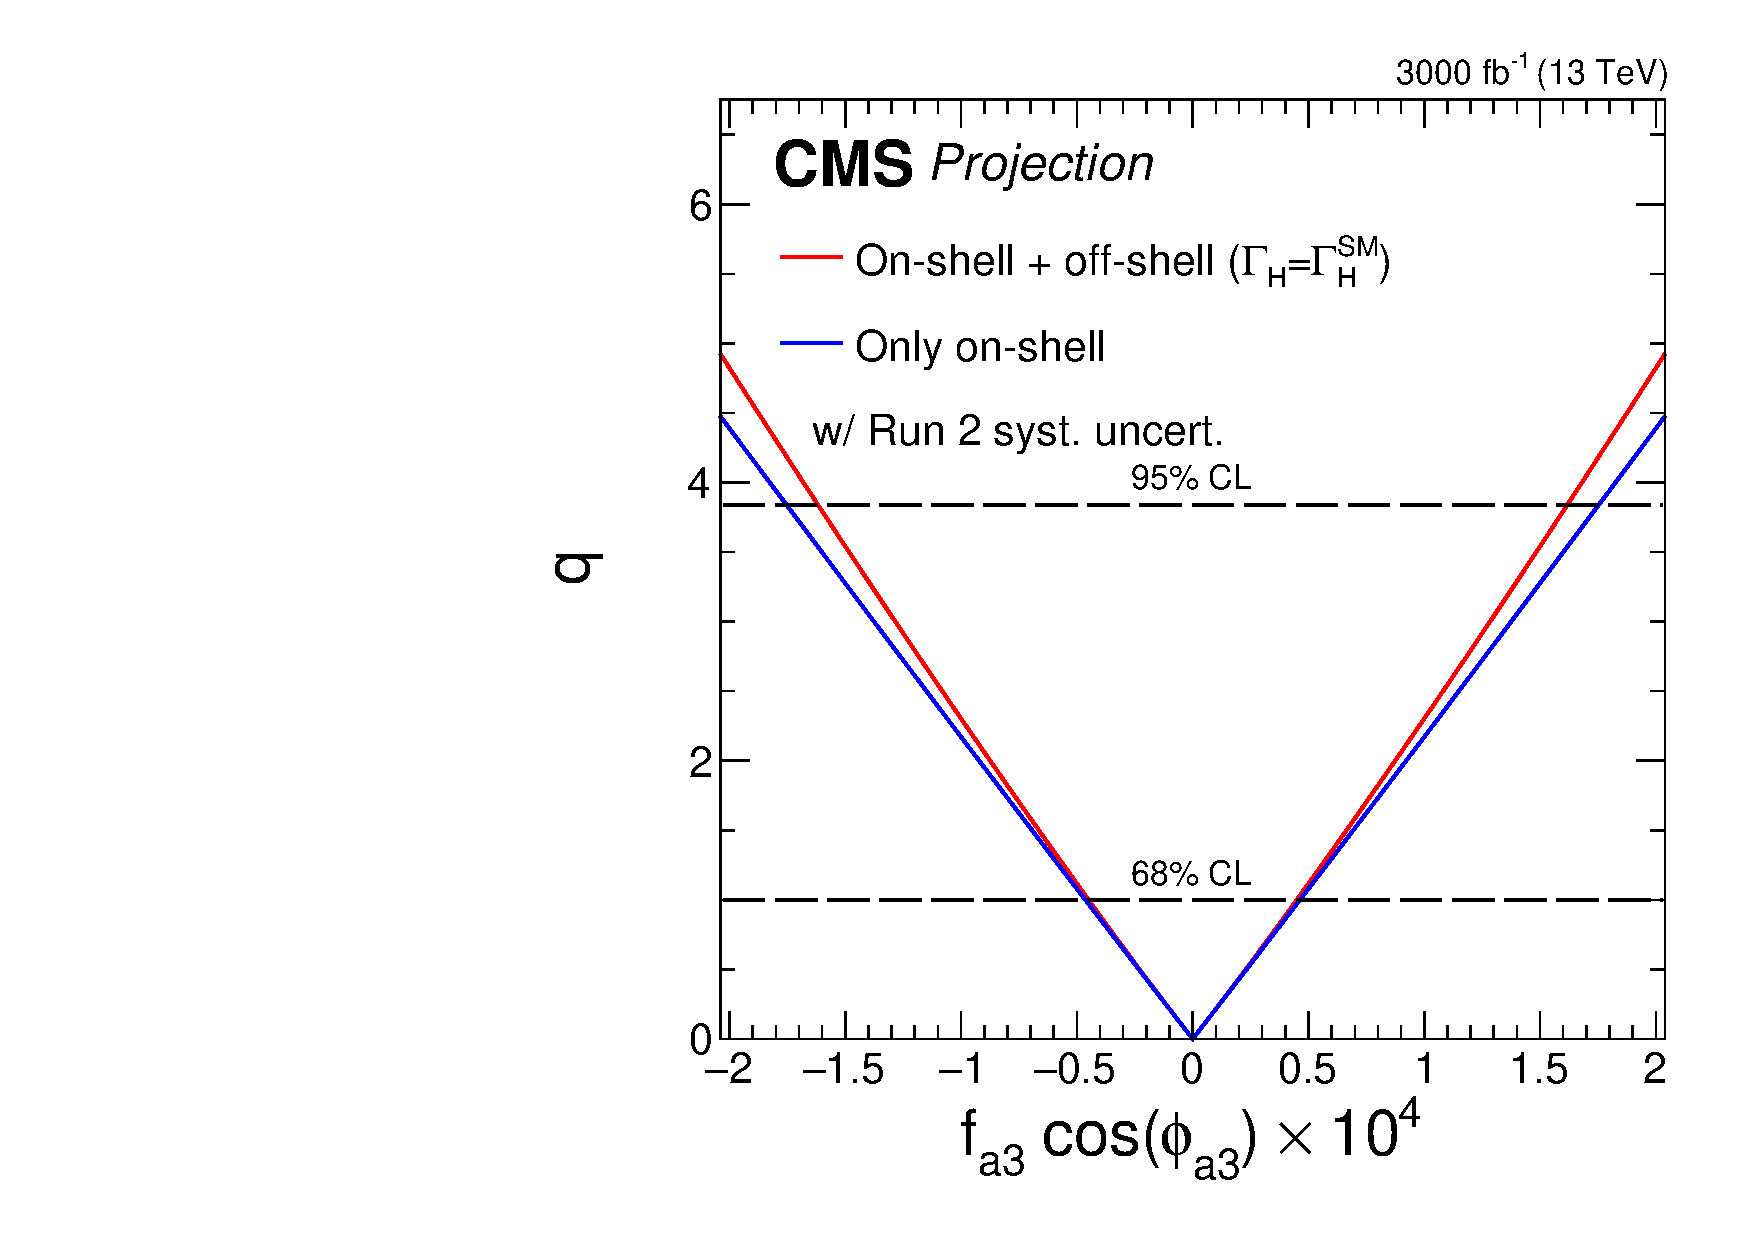
\includegraphics[width=0.90\textwidth]{section2/plots/hzz/cCompare_deltaNLLVSCMS_zz4l_fai1_Proj3000.pdf}
\caption
{
Likelihood scans for projections on \fcospAC{3} at $3000~\fbinv$~\cite{CMS-PAS-FTR-18-011}. The scans are shown using either the combination of \onshell and \offshell events (red) or only \onshell events (blue). The dashed lines represent the effect of removing all systematic uncertainties.
The dashed horizontal lines indicate the 68\% and 95\% CLs, and the \fcospAC{3} scans assume ${\GH}={\GHSM}$.
}
\label{fig:fa3-GH-projections}
\end{figure*}
%%%%%%%%%%%%%%%%%%%%%%%%%%%%%
